% Provenance (never printed): see sources/outline_sources.md (Year 1: crystal
% chemistry of minerals, silicates, solid solutions, mineral formulas, the main
% rock-forming minerals). Olivine curves in figdata/bachelor-1/solid_solution.py;
% the olivine analysis of the problem is invented (Fo about 82); exercise and
% problem values in the Book 3 scratch calculator calc/ch07.py.
\chapter{मुख्य शैल-निर्माता खनिज}\label{ch:b1:rock-forming-minerals}

एक ग्रेनाइट के काउंटरटॉप में तीन-चार प्रकार के कण दिखते हैं: काँच-जैसा धूसर स्फटिक, गुलाबी या सफ़ेद \omterm{def:b1:rock-forming-minerals:groups}{फ़ेल्सपार},
और काले \omterm{def:b1:rock-forming-minerals:groups}{अभ्रक} के पत्रक। समुद्र तट की रेत लगभग पूरी तरह स्फटिक है। बेसाल्ट में बिखरे छोटे हरे क्रिस्टल \omterm{def:b1:rock-forming-minerals:groups}{ओलिवीन}
हैं, और वही \omterm{def:b1:rock-forming-minerals:mineral}{खनिज}, थोड़े भिन्न संघटन में, ऊपरी प्रावार का अधिकांश बनाता है। मुट्ठी भर \omterm{def:b1:rock-forming-minerals:mineral}{खनिज} लगभग हर चट्टान
बनाते हैं, और उनमें लगभग सभी सिलिकेट हैं: ऑक्सीजन और सिलिकन, पर्पटी के दो सबसे प्रचुर तत्व, चतुष्फलकों में
जुड़े हैं जो कुछ सरल ढंगों से जुड़ते हैं। यह अध्याय बताता है कि यह जुड़ाव किसी सिलिकेट का सूत्र और उसकी
आदत कैसे तय करता है, एक क्रिस्टल में एक तत्व दूसरे की जगह कैसे लेता है ताकि एक \omterm{def:b1:rock-forming-minerals:mineral}{खनिज} एक संघटन न होकर संघटनों
का एक परास हो, एक रासायनिक विश्लेषण सूत्र कैसे बनता है, और मुख्य शैल-निर्माता \omterm{def:b1:rock-forming-minerals:mineral}{खनिज} क्या हैं। यह बेसाल्ट के
एक \omterm{def:b1:rock-forming-minerals:groups}{ओलिवीन} के विश्लेषण, पुनर्गणना और तौल के साथ समाप्त होता है।

\begin{recall}
क्रिस्टल एक ठोस है जिसके परमाणु एक जालक पर दोहराते हैं; एकक कोष्ठिका वह सबसे छोटा डिब्बा है जो दोहराता है, और
किसी आयन की समन्वय संख्या उसके विपरीत आवेश वाले निकटतम पड़ोसियों को गिनती है (रसायन विज्ञान, विश्वविद्यालय
वर्ष 1)। आयनिक त्रिज्याएँ आवेश और समन्वय पर निर्भर करती हैं। \omterm{def:b1:rock-forming-minerals:mineral}{खनिज} हाथ में उसकी आदत, विदलन, कठोरता और चमक से
पहचाना जाता है (पुस्तक 2, कक्षा 11)। पदार्थ की मात्रा मोल में गिनी जाती है, और मोलर द्रव्यमान एक मोल का द्रव्यमान
है (रसायन विज्ञान)।
\end{recall}

\section{खनिज क्या है}

\begin{definition}[खनिज]\label{def:b1:rock-forming-minerals:mineral}
एक \emph{खनिज}\index{खनिज} एक प्राकृतिक रूप से पाया जाने वाला ठोस है जिसकी एक निश्चित क्रिस्टल संरचना है और
जिसका रासायनिक संघटन या तो स्थिर है या निश्चित सीमाओं के भीतर बदलता है। लगभग सभी खनिज अकार्बनिक हैं।
\end{definition}

एक चट्टान, इसके विपरीत, एक या कई खनिजों (या काँच) के कणों का समुच्चय है: ग्रेनाइट स्फटिक, \omterm{def:b1:rock-forming-minerals:groups}{फ़ेल्सपार} और \omterm{def:b1:rock-forming-minerals:groups}{अभ्रक} है;
चूना-पत्थर मुख्यतः कैल्साइट है। परिभाषा के दोनों भाग स्वतंत्र हैं। खिड़की का काँच एक सिलिकेट का संघटन रखता है
पर उसकी कोई क्रिस्टल संरचना नहीं है: वह \omterm{def:b1:rock-forming-minerals:mineral}{खनिज} नहीं है, और न ही शीतल लावा का काँच। इसके विपरीत, वही संघटन कई
संरचनाओं में क्रिस्टलित हो सकता है, और हर संरचना एक अलग \omterm{def:b1:rock-forming-minerals:mineral}{खनिज} है।

\begin{definition}[बहुरूप]\label{def:b1:rock-forming-minerals:polymorph}
दो \omterm{def:b1:rock-forming-minerals:mineral}{खनिज} एक-दूसरे के \emph{बहुरूप}\index{बहुरूप} हैं जब उनका रासायनिक संघटन समान हो और उनकी क्रिस्टल संरचनाएँ भिन्न हों।
\end{definition}

कार्बन ग्रेफ़ाइट के रूप में क्रिस्टलित होता है, षट्कोणों की चादरों का एक ढेर, जिसका घनत्व \qty{2.16}{g.cm^{-3}} है,
और हीरे के रूप में, एक ढाँचा जिसमें हर परमाणु के चार पड़ोसी हैं, जिसका घनत्व \qty{3.51}{g.cm^{-3}} है। कैल्शियम
कार्बोनेट कैल्साइट (\qty{2.71}{g.cm^{-3}}) या ऐरागोनाइट (\qty{2.93}{g.cm^{-3}}) है; सिलिका स्फटिक
(\qty{2.65}{g.cm^{-3}}) या कोज़ाइट (\qty{2.93}{g.cm^{-3}}) है; \ce{Al2SiO5} काइनाइट (\qty{3.61}{g.cm^{-3}}),
एंडैलुसाइट (\qty{3.15}{g.cm^{-3}}) या सिलिमेनाइट (\qty{3.24}{g.cm^{-3}}) है।
% ledger: webmineral:polymorphs, hom:calcite, hom:quartz
हर युग्म में घना \omterm{def:b1:rock-forming-minerals:polymorph}{बहुरूप} वह है जो अधिक दाब पर बनता है: किसी दिए गए तापमान पर दाब बढ़ाने से कम आयतन वाली अवस्था
को बल मिलता है (रसायन विज्ञान, साम्य का विस्थापन)। एक किम्बरलाइट में हीरा और उल्कापिंड से टकराई चट्टान में कोज़ाइट
इसलिए केवल प्रावार की गहराई या एक प्रभाव में मिलने वाले दाब अभिलिखित करते हैं। तीन \ce{Al2SiO5} \omterm{def:b1:rock-forming-minerals:polymorph}{बहुरूप}, जिनके
स्थायित्व-क्षेत्र दाब-तापमान तल को आपस में बाँटते हैं, कायांतरण की परिस्थितियाँ पढ़ने के लिए प्रयुक्त होते हैं
(विश्वविद्यालय वर्ष 2)।

\section{सिलिकेट चतुष्फलक और उसके जोड़}

हर सामान्य सिलिकेट में, हर सिलिकन परमाणु एक नियमित चतुष्फलक के कोनों पर रखे चार ऑक्सीजन परमाणुओं के केंद्र में
होता है: रसायन विज्ञान से स्मरण की गई \ce{SiO4} इकाई। सिलिकन आयन छोटा है (चतुष्फलकीय समन्वय में
\qty{0.26}{\angstrom}) और ऑक्साइड आयन बड़ा, इसलिए उसके चारों ओर चार ऑक्सीजन आते हैं और इससे अधिक नहीं; सिलिकन-
ऑक्सीजन बंधन प्रबल और आंशिक रूप से सहसंयोजक है। एक अलग इकाई का आवेश $4 - 4\times2 = -4$ है।
% ledger: shannon:radii
चतुष्फलक अकेले खड़े हो सकते हैं, उनका आवेश उनके बीच की धातु धनायनों से संतुलित होता है, या वे कोने साझा कर
सकते हैं: दो चतुष्फलकों में साझा ऑक्सीजन एक \emph{सेतु} ऑक्सीजन है। दो चतुष्फलक कभी किनारा या फलक साझा नहीं
करते, जिससे दो सिलिकन बहुत पास आ जाते। सिलिकेट उस संख्या से वर्गीकृत होते हैं जितने कोने हर चतुष्फलक साझा
करता है (\cref{def:b1:rock-forming-minerals:silicate-classes})।

\begin{omfigure}
\tikzset{
  tup/.pic={\filldraw[fill=omLithLime, draw=black, line join=round] (0,0) -- (1,0) -- (0.5,0.866) -- cycle;
            \fill[omThm] (0.5,0.2887) circle (0.11);},
  tdn/.pic={\filldraw[fill=omLithLime, draw=black, line join=round] (0,0) -- (1,0) -- (0.5,-0.866) -- cycle;
            \fill[omThm] (0.5,-0.2887) circle (0.11);},
  linkpanel/.style={x=0.45cm, y=0.45cm, baseline=(current bounding box.south)}}
\setlength{\tabcolsep}{4pt}
\begin{tabular}{cccc}
% (a) the tetrahedron in perspective
\begin{tikzpicture}[linkpanel]
  \useasboundingbox (-1.2,-1.0) rectangle (6.0,4.4);
  \coordinate (T) at (2.2,3.7); \coordinate (L) at (0.3,0.5); \coordinate (R) at (4.1,0.1);
  \coordinate (B) at (3.3,2.1); \coordinate (C) at (2.475,1.6);
  \draw[densely dashed, gray] (L) -- (B) -- (R) (B) -- (T);
  \shade[ball color=omLithShale] (B) circle (0.42);
  \draw[gray] (C) -- (T) (C) -- (L) (C) -- (R) (C) -- (B);
  \shade[ball color=omThm!70] (C) circle (0.24);
  \draw[thick, line join=round] (T) -- (L) -- (R) -- cycle;
  \foreach \p in {T,L,R} \shade[ball color=omLithShale] (\p) circle (0.42);
  \node[right] at (4.5,0.1) {\scriptsize O};
  \node[right] at (2.6,3.8) {\scriptsize O};
  \draw[omThm] (C) -- (4.6,2.2) node[right] {\scriptsize Si};
\end{tikzpicture} &
% (b) nesosilicate: isolated tetrahedra
\begin{tikzpicture}[linkpanel]
  \useasboundingbox (-1.2,-1.0) rectangle (6.0,4.4);
  \pic at (0,0.3) {tup}; \pic at (2.4,0.3) {tup}; \pic at (4.0,1.9) {tdn};
  \pic at (1.2,2.4) {tdn}; \pic at (3.0,2.8) {tup};
\end{tikzpicture} &
% (c) sorosilicate: pairs
\begin{tikzpicture}[linkpanel]
  \useasboundingbox (-1.2,-1.0) rectangle (6.0,4.4);
  \pic at (0,0.9) {tup}; \pic at (1,0.9) {tdn};
  \pic at (2.6,2.6) {tup}; \pic at (3.6,2.6) {tdn};
\end{tikzpicture} &
% (d) cyclosilicate: a ring of six
\begin{tikzpicture}[linkpanel]
  \useasboundingbox (-1.2,-1.0) rectangle (6.0,4.4);
  \begin{scope}[shift={(2.4,1.7)}]
  \foreach \t in {0,60,...,300} {
    \filldraw[fill=omLithLime, draw=black, line join=round] (\t-30:1) -- (\t+30:1) -- (\t:1.732) -- cycle;
    \fill[omThm] (\t:1.155) circle (0.11);}
  \end{scope}
\end{tikzpicture} \\
{\small (क) \ce{SiO4} चतुष्फलक} & {\small (ख) \omterm{def:b1:rock-forming-minerals:silicate-classes}{नीसोसिलिकेट}} & {\small (ग) \omterm{def:b1:rock-forming-minerals:silicate-classes}{सोरोसिलिकेट}} & {\small (घ) \omterm{def:b1:rock-forming-minerals:silicate-classes}{साइक्लोसिलिकेट}} \\
 & {\scriptsize $s = 0$, \ce{SiO4}} & {\scriptsize $s = 1$, \ce{Si2O7}} & {\scriptsize $s = 2$, \ce{Si6O18}} \\[6pt]
% (e) single chain
\begin{tikzpicture}[linkpanel]
  \useasboundingbox (-0.6,-1.2) rectangle (7.6,4.6);
  \begin{scope}[shift={(0,1.5)}]
  \foreach \i in {0,...,3} \pic at (2*\i,0) {tup};
  \foreach \i in {0,...,2} \pic at (2*\i+1,0) {tdn};
  \end{scope}
\end{tikzpicture} &
% (f) double chain: two single chains joined through every other apex
\begin{tikzpicture}[linkpanel]
  \useasboundingbox (-0.6,-1.2) rectangle (7.6,4.6);
  \begin{scope}[shift={(0.5,0.4)}]
  \foreach \i in {0,...,3} {\pic at (2*\i,0) {tup}; \pic at (2*\i,1.732) {tdn};}
  \foreach \i in {0,...,2} {\pic at (2*\i+1,0) {tdn}; \pic at (2*\i+1,1.732) {tup};}
  \end{scope}
\end{tikzpicture} &
% (g) sheet
\begin{tikzpicture}[linkpanel]
  \useasboundingbox (-0.6,-1.2) rectangle (7.6,4.6);
  \foreach \j in {0,1,2} {
    \foreach \i in {0,1,2} {\pic at (2*\i+\j,1.732*\j) {tup};}
    \foreach \i in {0,1} {\pic at (2*\i+\j+1,1.732*\j) {tdn};}}
\end{tikzpicture} &
% (h) framework: a sheet whose apices point alternately up and down
\begin{tikzpicture}[linkpanel]
  \useasboundingbox (-0.6,-1.2) rectangle (7.6,4.6);
  \foreach \j in {0,1,2} {
    \foreach \i in {0,1,2} {\pic at (2*\i+\j,1.732*\j) {tup};}
    \foreach \i in {0,1} {\pic at (2*\i+\j+1,1.732*\j) {tdn};}}
  \foreach \j in {0,1,2} \foreach \i in {0,1} {
    \filldraw[fill=white, draw=omThm, thick] (2*\i+\j+1.5,1.732*\j-0.2887) circle (0.17);}
\end{tikzpicture} \\
{\small (ङ) एकल शृंखला} & {\small (च) द्वि-शृंखला} & {\small (छ) परत} & {\small (ज) ढाँचा} \\
{\scriptsize $s = 2$, \ce{SiO3}} & {\scriptsize $s = 2$ और $3$, \ce{Si4O11}} & {\scriptsize $s = 3$, \ce{Si2O5}} & {\scriptsize $s = 4$, \ce{SiO2}} \\
\end{tabular}
\medskip

{\small \ce{SiO4} चतुष्फलक (क) और चतुष्फलकों के जुड़ने के ढंग, ऊपर से देखे गए: हर त्रिभुज एक चतुष्फलक का आधार है,
जिसके कोनों पर तीन ऑक्सीजन हैं, चौथा बिंदु के ऊपर है, जो सिलिकन को चिह्नित करता है। छूने वाले कोने साझा
ऑक्सीजन हैं; $s$ वह संख्या है जितने कोने हर चतुष्फलक साझा करता है। ढाँचे (ज) में शीर्ष ऑक्सीजन (खुले वृत्त: नीचे
की ओर; बिंदु: ऊपर की ओर) ऊपर और नीचे की परतों के साथ भी साझा हैं।}
\end{omfigure}

\begin{definition}[सिलिकेट वर्ग]\label{def:b1:rock-forming-minerals:silicate-classes}
सिलिकेट इस आधार पर वर्गीकृत होते हैं कि उनके \ce{SiO4} चतुष्फलक कैसे जुड़ते हैं। एक \emph{नीसोसिलिकेट}\index{नीसोसिलिकेट}
में चतुष्फलक अलग होते हैं; एक \emph{सोरोसिलिकेट}\index{सोरोसिलिकेट} में वे एक साझा ऑक्सीजन से जोड़ों में जुड़े
होते हैं; एक \emph{साइक्लोसिलिकेट}\index{साइक्लोसिलिकेट} में वे बंद वलय बनाते हैं, जिनमें हर एक दो कोने साझा करता
है; एक \emph{इनोसिलिकेट}\index{इनोसिलिकेट} में वे अंतहीन शृंखलाएँ बनाते हैं, एकल (हर चतुष्फलक दो कोने साझा करता हुआ)
या द्वि-शृंखला (दो एकल शृंखलाएँ साथ-साथ जुड़ी हुईं, आधे चतुष्फलक तीन कोने साझा करते हुए); एक
\emph{फ़िलोसिलिकेट}\index{फ़िलोसिलिकेट} में वे अंतहीन परतें बनाते हैं, हर एक तीन कोने साझा करता हुआ; एक
\emph{टेक्टोसिलिकेट}\index{टेक्टोसिलिकेट} में वे त्रि-विमीय ढाँचा बनाते हैं, हर एक चारों कोने साझा करता हुआ।
\end{definition}

\begin{proposition}[सिलिकन और ऑक्सीजन का अनुपात]\label{prop:b1:rock-forming-minerals:si-o}
यदि किसी सिलिकेट के हर \ce{SiO4} चतुष्फलक, अपने चार कोनों में से, औसतन $s$ दूसरे चतुष्फलकों के साथ साझा करता
है, और हर साझा ऑक्सीजन ठीक दो चतुष्फलकों का है, तो सिलिकेट जाल में प्रति सिलिकन $4 - s/2$ ऑक्सीजन होते हैं, और
प्रति सिलिकन $s - 4$ का आवेश वहन करता है।
\end{proposition}

\begin{proof}
चतुष्फलक-दर-चतुष्फलक ऑक्सीजन गिनिए। $s_i$ साझा कोनों वाला एक चतुष्फलक अपने $4 - s_i$ अ-साझा ऑक्सीजन पूरे
स्वामित्व में रखता है, और अपने $s_i$ साझा ऑक्सीजनों में से हर एक का आधा, क्योंकि हर एक को पड़ोसी चतुष्फलक
फिर गिनता है: वह $4 - s_i + s_i/2 = 4 - s_i/2$ ऑक्सीजन देता है। $N$ चतुष्फलकों पर जोड़ने और $N$ से भाग देने पर
प्रति सिलिकन $4 - s/2$ ऑक्सीजन मिलते हैं, जहाँ $s$, $s_i$ का माध्य है। हर सिलिकन $+4$ और हर ऑक्सीजन $-2$
का आवेश लाता है, अतः प्रति सिलिकन आवेश $4 - 2(4 - s/2) = s - 4$ है।
\end{proof}

प्रस्ताव हर वर्ग के आयन को एक बार में देता है। अलग चतुष्फलक ($s = 0$): \ce{SiO4^{4-}}। जोड़े ($s = 1$): $4 - 1/2 = 7/2$,
यानी \ce{Si2O7^{6-}}। वलय और एकल शृंखलाएँ ($s = 2$): \ce{SiO3^{2-}}, छह के वलय के लिए \ce{Si6O18^{12-}} लिखा जाता है,
शृंखला के दो चतुष्फलकों के लिए \ce{Si2O6^{4-}}। द्वि-शृंखलाएँ (आधे $s = 2$, आधे $s = 3$, इसलिए $s = 5/2$):
$4 - 5/4 = 11/4$, \ce{Si4O11^{6-}}। परतें ($s = 3$): \ce{Si2O5^{2-}}। ढाँचे ($s = 4$): \ce{SiO2}, उदासीन --- स्फटिक
केवल सिलिकन और ऑक्सीजन का ढाँचा है। चतुष्फलक जितना अधिक साझा करते हैं, संतुलित करने के लिए उतना कम आवेश
होता है और उतने ही कम धातु धनायन: \omterm{def:b1:rock-forming-minerals:groups}{ओलिवीन} \ce{Mg2SiO4} में प्रति सिलिकन दो धातु आयन हैं, एन्स्टेटाइट जैसे एक \omterm{def:b1:rock-forming-minerals:groups}{पाइरॉक्सीन}
\ce{Mg2Si2O6} में एक, और स्फटिक में कोई नहीं।

संरचना क्रिस्टल को भी आकार देती है। एक परत सिलिकेट अपनी परतों के बीच आसानी से टूटता है, जहाँ बंधन दुर्बल हैं:
\omterm{def:b1:rock-forming-minerals:groups}{अभ्रक} पतले लचीले पत्रकों में छिलते हैं। शृंखला सिलिकेट अपनी शृंखलाओं के समांतर, दो तलों के साथ विदलित होते
हैं, जिनके बीच का कोण इस पर निर्भर है कि शृंखलाएँ कैसे सटती हैं: \omterm{def:b1:rock-forming-minerals:groups}{पाइरॉक्सीन} में लगभग \ang{87} और \ang{93}, जिनकी
शृंखलाएँ सँकरी हैं; \omterm{def:b1:rock-forming-minerals:groups}{एम्फ़ीबोल} में \ang{56} और \ang{124}, जिनकी द्वि-शृंखलाएँ चौड़ी हैं। टूटे क्रिस्टल पर, या \omterm{def:b1:field-lab-methods-1:thin-section}{पतली
काट} में देखे गए ये दो विदलन-कोण, दोनों समूहों को अलग पहचानने का क्लासिक तरीका हैं।
% ledger: hom:diopside, hom:mg-hornblende

\section{आयनिक प्रतिस्थापन और ठोस विलयन}

एक क्रिस्टल स्थलों का एक समुच्चय है, और एक स्थल अपने आकार और अपने आवेश से परिभाषित होता है, किसी एक तत्व से नहीं।
एक सही आकार और आवेश वाला आयन बढ़ते क्रिस्टल में दूसरे की जगह ले सकता है, और कोई चट्टान इतनी शुद्ध नहीं कि
केवल एक तत्व दे सके।

\begin{definition}[आयनिक प्रतिस्थापन, युग्मित प्रतिस्थापन]\label{def:b1:rock-forming-minerals:substitution}
एक \emph{आयनिक प्रतिस्थापन}\index{आयनिक प्रतिस्थापन} एक क्रिस्टल संरचना के किसी स्थल में, संरचना बदले बिना, एक
आयन का समान त्रिज्या वाले दूसरे आयन से स्थान लेना है। एक \emph{युग्मित
प्रतिस्थापन}\index{युग्मित प्रतिस्थापन} दो भिन्न स्थलों पर प्रतिस्थापनों का एक युग्म है जिनके आवेश-परिवर्तन एक-दूसरे
को निरस्त करते हैं, ताकि क्रिस्टल उदासीन रहे।
\end{definition}

गोल्डश्मिट के दो अनुभवजन्य नियम बताते हैं कि कौन-से प्रतिस्थापन संभव हैं। त्रिज्याएँ निकट होनी चाहिए: प्रतिस्थापन
मुक्त होता है जब वे लगभग \qty{15}{\percent} से कम अंतर रखती हैं, लगभग 15 और \qty{30}{\percent} के बीच सीमित होता है,
और उससे आगे दुर्लभ। आवेश एक इकाई से अधिक नहीं भिन्न होने चाहिए, और आवेश का अंतर संरचना में कहीं और क्षतिपूरित
होना चाहिए। \omterm{def:b1:rock-forming-minerals:groups}{ओलिवीन} के षट्भुजीय स्थल में \ce{Mg^{2+}} (\qty{0.72}{\angstrom}) मुक्त रूप से \ce{Fe^{2+}}
(\qty{0.78}{\angstrom}, \qty{8}{\percent} बड़ा) और \ce{Ni^{2+}} (\qty{0.69}{\angstrom}) से, थोड़ा \ce{Mn^{2+}}
(\qty{0.83}{\angstrom}) से, और मुश्किल से \ce{Ca^{2+}} (\qty{1.00}{\angstrom}, \qty{39}{\percent} बड़ा) से बदला जाता है।
% ledger: goldschmidt:size, shannon:radii
ये नियम मार्गदर्शक हैं: तापमान संभव परास को चौड़ा करता है, क्योंकि एक गर्म क्रिस्टल अधिक विकृति सहता है; इसीलिए
ऊँचे तापमान पर उगा \omterm{def:b1:rock-forming-minerals:mineral}{खनिज} अक्सर उसी \omterm{def:b1:rock-forming-minerals:mineral}{खनिज} से अधिक बेमेल आयन रखता है जो ठंडा उगा हो।

\begin{definition}[ठोस विलयन, अंत्य-सदस्य]\label{def:b1:rock-forming-minerals:solid-solution}
एक \emph{ठोस विलयन}\index{ठोस विलयन (खनिज)} वह \omterm{def:b1:rock-forming-minerals:mineral}{खनिज} है जिसमें एक या अधिक संरचनात्मक स्थल, सतत बदलते अनुपातों
में, दो या अधिक आयनों से भरे होते हैं। एक ठोस विलयन के \emph{अंत्य-सदस्य}\index{अंत्य-सदस्य} उसकी सीमाओं पर के
संघटन हैं, जिनमें हर परिवर्ती स्थल केवल एक आयन से भरा होता है; एक मध्यवर्ती संघटन अंत्य-सदस्यों के मोल-
अंशों से दिया जाता है।
\end{definition}

\omterm{def:b1:rock-forming-minerals:groups}{ओलिवीन} फ़ॉर्स्टेराइट \ce{Mg2SiO4} (Fo) और फ़ायलाइट \ce{Fe2SiO4} (Fa) के बीच का \omterm{def:b1:rock-forming-minerals:solid-solution}{ठोस विलयन} है, एक \omterm{def:b1:rock-forming-minerals:solid-solution}{अंत्य-सदस्य} से
दूसरे तक पूर्ण: एक \omterm{def:b1:rock-forming-minerals:groups}{ओलिवीन} जिसके षट्भुजीय स्थलों का \qty{82}{\percent} मैग्नीशियम से और \qty{18}{\percent} लोहे से
भरा है, $\text{Fo}_{82}$, या \ce{(Mg_{0.82}Fe_{0.18})2SiO4} लिखा जाता है। \omterm{def:b1:rock-forming-minerals:groups}{गार्नेट}, \omterm{def:b1:rock-forming-minerals:groups}{पाइरॉक्सीन}, \omterm{def:b1:rock-forming-minerals:groups}{एम्फ़ीबोल} और \omterm{def:b1:rock-forming-minerals:groups}{अभ्रक} उसी
ढंग से \omterm{def:b1:rock-forming-minerals:solid-solution}{ठोस विलयन} हैं। \omterm{def:b1:rock-forming-minerals:groups}{प्लैजियोक्लेज़} \omterm{def:b1:rock-forming-minerals:groups}{फ़ेल्सपार} एक भिन्न प्रकार का \omterm{def:b1:rock-forming-minerals:solid-solution}{ठोस विलयन} है, एल्बाइट \ce{NaAlSi3O8} (Ab) और
एनॉर्थाइट \ce{CaAl2Si2O8} (An) के बीच। सोडियम और कैल्शियम की त्रिज्याएँ लगभग समान हैं
(षट्भुजीय समन्वय में \qty{1.02}{\angstrom} और \qty{1.00}{\angstrom}) पर उनके आवेश भिन्न हैं; हर कैल्शियम जो प्रवेश
करता है, उसके साथ एक चतुष्फलक में सिलिकन की जगह लेता एक एल्युमिनियम होना चाहिए:
% ledger: shannon:radii
\[
  \mathrm{Na^{+}} + \mathrm{Si^{4+}} \;\rightleftharpoons\; \mathrm{Ca^{2+}} + \mathrm{Al^{3+}},
\]
एक \omterm{def:b1:rock-forming-minerals:substitution}{युग्मित प्रतिस्थापन} जो कुल आवेश अपरिवर्तित छोड़ता है।
एल्युमिनियम एक चतुष्फलक में प्रवेश कर सकता है क्योंकि वह पर्याप्त छोटा है (चतुष्फलकीय समन्वय में
\qty{0.39}{\angstrom}); सिलिकेटों में सिलिकन के लिए यह सबसे आम प्रतिस्थापन है।

\begin{omfigure}
\begin{tikzpicture}[x=1cm, y=1cm,
  site/.style={draw, minimum width=1.25cm, minimum height=0.75cm, font=\small},
  asite/.style={site, fill=omLithGranite!60},
  tsite/.style={site, fill=omLithLime}]
\node[font=\small\bfseries, anchor=east] at (-0.4,1.6) {एल्बाइट};
\node[asite] (a0) at (0.5,1.6) {$\mathrm{Na^{+}}$};
\node[tsite] (a1) at (2.2,1.6) {$\mathrm{Al^{3+}}$};
\node[tsite] (a2) at (3.55,1.6) {$\mathrm{Si^{4+}}$};
\node[tsite] (a3) at (4.9,1.6) {$\mathrm{Si^{4+}}$};
\node[tsite] (a4) at (6.25,1.6) {$\mathrm{Si^{4+}}$};
\node[anchor=west, font=\small] at (7.2,1.6) {$1 + 3 + 3\times4 = +16$, \ce{O8} के साथ: $-16$};
\node[font=\small\bfseries, anchor=east] at (-0.4,-0.6) {एनॉर्थाइट};
\node[asite] (b0) at (0.5,-0.6) {$\mathrm{Ca^{2+}}$};
\node[tsite] (b1) at (2.2,-0.6) {$\mathrm{Al^{3+}}$};
\node[tsite] (b2) at (3.55,-0.6) {$\mathrm{Al^{3+}}$};
\node[tsite] (b3) at (4.9,-0.6) {$\mathrm{Si^{4+}}$};
\node[tsite] (b4) at (6.25,-0.6) {$\mathrm{Si^{4+}}$};
\node[anchor=west, font=\small] at (7.2,-0.6) {$2 + 2\times3 + 2\times4 = +16$, \ce{O8} के साथ: $-16$};
\draw[-{Stealth}, omThm, thick] (a0) -- node[left, font=\scriptsize] {$+1$} (b0);
\draw[-{Stealth}, omThm, thick] (a2) -- node[right, font=\scriptsize] {$-1$} (b2);
\node[font=\scriptsize] at (0.5,2.35) {बड़ा स्थल};
\node[font=\scriptsize] at (4.22,2.35) {चार चतुष्फलकीय स्थल};
\end{tikzpicture}

{\small \omterm{def:b1:rock-forming-minerals:groups}{प्लैजियोक्लेज़} में \omterm{def:b1:rock-forming-minerals:substitution}{युग्मित प्रतिस्थापन}। बड़े स्थल में एक सोडियम को कैल्शियम से बदलने पर एक धनात्मक आवेश
जुड़ता है; एक चतुष्फलक में एक सिलिकन को एल्युमिनियम से बदलने पर एक आवेश हटता है। हर मध्यवर्ती \omterm{def:b1:rock-forming-minerals:groups}{प्लैजियोक्लेज़}
$\mathrm{Na}_{1-x}\mathrm{Ca}_x\mathrm{Al}_{1+x}\mathrm{Si}_{3-x}\mathrm{O}_8$ उदासीन है।}
\end{omfigure}

एक \omterm{def:b1:rock-forming-minerals:solid-solution}{ठोस विलयन} के गुण उसके संघटन के साथ बदलते हैं, और यही उन्हें उपयोगी बनाता है: एक मापा घनत्व, एक अपवर्तनांक या
एक एकक-कोष्ठिका आयाम संघटन देता है। सबसे सरल प्रतिरूप \omterm{def:b1:rock-forming-minerals:solid-solution}{ठोस विलयन} को आयतन में एक आदर्श मिश्रण मानता है: $\text{Fo}_x$
का एक मोल, $x$ मोल फ़ॉर्स्टेराइट और $1 - x$ मोल फ़ायलाइट के आयतन लेता है। यह एक प्रतिरूप है, जिसकी मापनों से
तुलना करनी है, और यह घनत्व के बारे में पहले से कुछ अप्रत्याशित बताता है।

\begin{proposition}[एक आदर्श ठोस विलयन का मोलर आयतन और घनत्व]\label{prop:b1:rock-forming-minerals:ideal-mixing}
मान लीजिए दो अंत्य-सदस्यों के मोलर द्रव्यमान $M_1$, $M_2$ और मोलर आयतन $V_1 = M_1/\rho_1$, $V_2 = M_2/\rho_2$ हैं।
\omterm{def:b1:rock-forming-minerals:solid-solution}{अंत्य-सदस्य} 1 के मोल-अंश $x$ वाले एक \omterm{def:b1:rock-forming-minerals:solid-solution}{ठोस विलयन} में मोलर द्रव्यमान
$M(x) = x M_1 + (1 - x) M_2$ है। यदि मोलर आयतन $V(x) = x V_1 + (1 - x) V_2$ है (आदर्श मिश्रण), तो घनत्व
\[
  \rho(x) = \frac{x M_1 + (1 - x) M_2}{x V_1 + (1 - x) V_2},
\]
है, जो $\rho_1$ के बराबर है, $x = 1$ पर, और $\rho_2$ के बराबर है, $x = 0$ पर, और $x$ का एक रैखिक फलन केवल तब है जब
$V_1 = V_2$ या $\rho_1 = \rho_2$।
\end{proposition}

\begin{proof}
\omterm{def:b1:rock-forming-minerals:solid-solution}{ठोस विलयन} के एक मोल में पहले सूत्र-एकक के $x$ मोल और दूसरे के $1 - x$ मोल हैं; उसका द्रव्यमान $x M_1 + (1 - x) M_2$
है, उसका आयतन परिकल्पना से $V(x)$ है, और $\rho = M/V$। $x = 1$ पर $\rho = M_1/V_1 = \rho_1$; $x = 0$ पर $\rho = \rho_2$।
यदि $V_1 = V_2$, तो $\rho = M(x)/V_1$ रैखिक है। अन्यथा $\rho = (a + bx)/(c + dx)$ लिखिए, जहाँ $d = V_1 - V_2 \ne 0$।
यदि वह रैखिक, $p + qx$, होता, तो $a + bx = (c + dx)(p + qx)$ सभी $x$ के लिए होता, और $x^2$ का गुणांक
$qd = 0$ देता, अतः $q = 0$: तब $\rho$ स्थिर होता, $\rho_1 = \rho_2$। विलोमतः, समान \omterm{def:b1:rock-forming-minerals:solid-solution}{अंत्य-सदस्य} घनत्व $\rho$ को
स्थिर बनाते हैं।
\end{proof}

\omterm{def:b1:rock-forming-minerals:groups}{ओलिवीन} के लिए, फ़ॉर्स्टेराइट के लिए मापे गए घनत्व \qty{3.275}{g.cm^{-3}} और फ़ायलाइट के लिए \qty{4.392}{g.cm^{-3}} के साथ,
और मोलर द्रव्यमान \qty{140.691}{g.mol^{-1}} और \qty{203.771}{g.mol^{-1}} के साथ, मोलर आयतन
\qty{42.96}{cm^3.mol^{-1}} और \qty{46.40}{cm^3.mol^{-1}} हैं: मैग्नीशियम को बड़े लौह-आयन से बदलने पर क्रिस्टल
\qty{8}{\percent} फूल जाता है, और उसके द्रव्यमान में \qty{45}{\percent} जोड़ता है। घनत्व वक्र अंत्य-सदस्यों को जोड़ने
वाली सीधी रेखा से थोड़ा ऊपर रहता है, \qty{0.02}{g.cm^{-3}} तक
(\cref{exo:b1:rock-forming-minerals:10}): रैखिक अंतर्वेशन निकट है, पर सटीक नहीं।
% ledger: hom:forsterite, hom:fayalite, ciaaw:Mg, ciaaw:Fe, ciaaw:Si, ciaaw:O

\begin{omfigure}
\begin{tikzpicture}
\begin{axis}[name=vol, width=0.48\linewidth, height=5.2cm,
  xmin=0, xmax=100, ymin=42.5, ymax=46.8, xtick={0,20,...,100},
  tick label style={font=\scriptsize}, label style={font=\small},
  xlabel={फ़ॉर्स्टेराइट अंश (mol\,\%)}, ylabel={मोलर आयतन (\si{cm^3.mol^{-1}})},
  yticklabel style={/pgf/number format/fixed, /pgf/number format/precision=1}]
\addplot[omThm, thick] table[x=x_fo, y=V] {figdata/out/bachelor-1-solid_solution-curve.dat};
\node[font=\scriptsize, anchor=north west] at (axis cs:3,45.55) {फ़ायलाइट};
\node[font=\scriptsize, anchor=north east] at (axis cs:97,42.95) {फ़ॉर्स्टेराइट};
\end{axis}
\begin{axis}[at={(vol.east)}, anchor=west, xshift=1.3cm, width=0.48\linewidth, height=5.2cm,
  xmin=0, xmax=100, ymin=3.2, ymax=4.45, xtick={0,20,...,100},
  tick label style={font=\scriptsize}, label style={font=\small},
  xlabel={फ़ॉर्स्टेराइट अंश (mol\,\%)}, ylabel={घनत्व (\si{g.cm^{-3}})},
  yticklabel style={/pgf/number format/fixed, /pgf/number format/precision=1}]
\addplot[gray, densely dashed] table[x=x_fo, y=rho_lin] {figdata/out/bachelor-1-solid_solution-curve.dat};
\addplot[omThm, thick] table[x=x_fo, y=rho] {figdata/out/bachelor-1-solid_solution-curve.dat};
\end{axis}
\end{tikzpicture}

{\small \omterm{def:b1:rock-forming-minerals:groups}{ओलिवीन} \omterm{def:b1:rock-forming-minerals:solid-solution}{ठोस विलयन}, फ़ॉर्स्टेराइट और फ़ायलाइट के एक आदर्श मिश्रण के रूप में, उनके मापे गए घनत्वों से। बाएँ:
मोलर आयतन, संघटन में रैखिक। दाएँ: घनत्व (ठोस), अंत्य-सदस्यों के बीच की सीधी रेखा (बिंदुरेखा) से थोड़ा ऊपर।}
\end{omfigure}

\section{खनिज सूत्र}

\begin{definition}[संरचनात्मक सूत्र, Mg संख्या]\label{def:b1:rock-forming-minerals:formula}
किसी \omterm{def:b1:rock-forming-minerals:mineral}{खनिज} का \emph{संरचनात्मक सूत्र}\index{संरचनात्मक सूत्र (खनिज)} ऑक्सीजन परमाणुओं की एक निश्चित संख्या के लिए
हर तत्व के परमाणुओं की संख्या और हर एक द्वारा घेरे गए स्थल देता है, जिसमें एक ही स्थल साझा करने वाले आयन एक साथ
लिखे जाते हैं: \omterm{def:b1:rock-forming-minerals:groups}{ओलिवीन} $\mathrm{(Mg, Fe)_2SiO_4}$, एक \omterm{def:b1:rock-forming-minerals:groups}{प्लैजियोक्लेज़}
$\mathrm{(Na_{0.5}Ca_{0.5})(Al_{1.5}Si_{2.5})O_8}$। किसी \omterm{def:b1:rock-forming-minerals:mineral}{खनिज} या चट्टान की \emph{Mg संख्या}\index{Mg संख्या} है
\[
  \mathrm{Mg\#} = 100\,\frac{\mathrm{Mg}}{\mathrm{Mg} + \mathrm{Fe^{2+}}},
\]
परमाणुओं की संख्या मोलों में (या प्रति सूत्र-एकक) गिनी जाती है।
\end{definition}

एक पॉलिश की गई \omterm{def:b1:field-lab-methods-1:thin-section}{पतली काट} पर एक इलेक्ट्रॉन माइक्रोप्रोब से बना \omterm{def:b1:rock-forming-minerals:mineral}{खनिज} का एक रासायनिक विश्लेषण (\cref{ch:b1:field-lab-methods-1})
सूत्र नहीं देता: वह हर तत्व का द्रव्यमान देता है, जो परिपाटी से उसके ऑक्साइड के द्रव्यमान के रूप में, नमूने के द्रव्यमान
के प्रतिशत में दिया जाता है। इन प्रतिशतों को सूत्र में बदलना एक नियमित गणना है।

\begin{method}[स्थिर ऑक्सीजन संख्या पर विश्लेषण की पुनर्गणना]\label{met:b1:rock-forming-minerals:recalculation}
मान लीजिए एक विश्लेषण ऑक्साइडों को भार प्रतिशत में देता है, और \omterm{def:b1:rock-forming-minerals:mineral}{खनिज} का प्रति सूत्र-एकक $n_O$ ऑक्सीजन है (\omterm{def:b1:rock-forming-minerals:groups}{ओलिवीन}
के लिए 4, \omterm{def:b1:rock-forming-minerals:groups}{फ़ेल्सपार} के लिए 8, \omterm{def:b1:rock-forming-minerals:groups}{पाइरॉक्सीन} के लिए 6, \omterm{def:b1:rock-forming-minerals:groups}{गार्नेट} के लिए 12)।
\begin{enumerate}
  \item हर ऑक्साइड के भार प्रतिशत को उसके मोलर द्रव्यमान से भाग दीजिए: इससे \qty{100}{g} \omterm{def:b1:rock-forming-minerals:mineral}{खनिज} में ऑक्साइड के मोल मिलते हैं।
  \item ऑक्साइड में ऑक्सीजन की संख्या से गुणा कीजिए (\ce{SiO2} के लिए 2, \ce{Al2O3} के लिए 3, \ce{MgO} के लिए 1) ताकि
        ऑक्सीजन के मोल मिलें, और ऑक्साइड में धनायनों की संख्या से (\ce{Al2O3} और \ce{Na2O} के लिए 2, \ce{SiO2} के लिए 1)
        ताकि धनायन के मोल मिलें।
  \item ऑक्सीजन के मोल जोड़िए, और गुणक $f = n_O / \sum(\text{मोल O})$ परिकलित कीजिए।
  \item हर धनायन के मोलों को $f$ से गुणा कीजिए: परिणाम प्रति सूत्र-एकक हर तत्व के परमाणु हैं।
  \item धनायनों को स्थलों में बाँटिए (सिलिकन और इतना एल्युमिनियम कि चतुष्फलक भर जाएँ, बाकी बड़े स्थलों में), और जाँचिए कि
        हर स्थल में आदर्श सूत्र के परमाणुओं की संख्या है।
\end{enumerate}
\end{method}

कार्य किया हुआ उदाहरण: एक \omterm{def:b1:rock-forming-minerals:groups}{ओलिवीन} जिसमें \qty{40.80}{\percent} \ce{SiO2}, \qty{49.40}{\percent} \ce{MgO} और
\qty{9.80}{\percent} \ce{FeO} है। मोलर द्रव्यमान \num{60.083}, \num{40.304} और \qty{71.844}{g.mol^{-1}} के साथ,
\qty{100}{g} में मोल $0.67906$, $1.22568$ और $0.13641$ हैं; ऑक्सीजन $2\times0.67906 + 1.22568 + 0.13641 = 2.72021$ हैं,
और गुणक $f = 4/2.72021 = 1.47047$ है। प्रति चार ऑक्सीजन: Si \num{0.999}, Mg \num{1.802}, Fe \num{0.201}। चतुष्फलकीय स्थल
\num{0.999} परमाणु रखता है और अष्टफलकीय स्थल $1.802 + 0.201 = 2.003$, 1 और 2 के बहुत निकट: विश्लेषण अच्छा है, और \omterm{def:b1:rock-forming-minerals:groups}{ओलिवीन}
\ce{(Mg_{1.80}Fe_{0.20})SiO4} है, $\text{Fo}_{90}$, 90 की \omterm{def:b1:rock-forming-minerals:formula}{Mg संख्या} के साथ। ध्यान दीजिए कि आवेश अपने आप $2n_O = 8$ तक
जुड़ते हैं, चाहे विश्लेषण कुछ भी हो, जब तक हर धनायन अपने ऑक्साइड का आवेश रखे: पुनर्गणना स्वयं सूत्र को उदासीन
बनाती है। स्थल-योग असली परीक्षा हैं।
% ledger: ciaaw:Si, ciaaw:Mg, ciaaw:Fe, ciaaw:O

चुने गए ऑक्सीजन-संख्या पर धनायनों का योग बहुत बड़ा हो तो यह बताता है कि कुछ लोहा \ce{Fe^{3+}} है, जो प्रति परमाणु
उतनी अधिक ऑक्सीजन लाता है जितनी विश्लेषण ने मानी थी (\cref{exo:b1:rock-forming-minerals:12}); योग बहुत छोटा हो, या
कुल \qty{100}{\percent} से बहुत नीचे, तो बताता है कि कुछ नहीं विश्लेषित हुआ --- एक \omterm{def:b1:rock-forming-minerals:groups}{एम्फ़ीबोल} या \omterm{def:b1:rock-forming-minerals:groups}{अभ्रक} में पानी, एक कार्बोनेट
में कार्बन डाइऑक्साइड। जलयुक्त खनिजों की इसलिए उनकी निर्जल ऑक्सीजनों पर पुनर्गणना होती है: एक \omterm{def:b1:rock-forming-minerals:groups}{एम्फ़ीबोल} के लिए 23,
जिसके सूत्र में \ce{O22(OH)2} है, और एक \omterm{def:b1:rock-forming-minerals:groups}{अभ्रक} के लिए 22, जिसकी दोगुनी सूत्र-इकाई में \ce{O20(OH)4} है।

\section{मुख्य शैल-निर्माता खनिज}

\begin{definition}[मुख्य खनिज समूह]\label{def:b1:rock-forming-minerals:groups}
\emph{ओलिवीन}\index{ओलिवीन} \omterm{def:b1:rock-forming-minerals:silicate-classes}{नीसोसिलिकेट} \omterm{def:b1:rock-forming-minerals:solid-solution}{ठोस विलयन} \ce{(Mg,Fe)2SiO4} है। \emph{गार्नेट}\index{गार्नेट} घनीय नीसोसिलिकेटों
का एक समूह है $\mathrm{X_3Y_2(SiO_4)_3}$, जिसमें X एक द्विसंयोजी आयन (Mg, Fe, Mn, Ca) है, Y एक त्रिसंयोजी (Al, Fe, Cr)।
एक \emph{पाइरॉक्सीन}\index{पाइरॉक्सीन} एकल-शृंखला \omterm{def:b1:rock-forming-minerals:silicate-classes}{इनोसिलिकेट} है $\mathrm{XYSi_2O_6}$; एक
\emph{एम्फ़ीबोल}\index{एम्फ़ीबोल} हाइड्रॉक्सिल वाला द्वि-शृंखला \omterm{def:b1:rock-forming-minerals:silicate-classes}{इनोसिलिकेट} है, लगभग $\mathrm{A_{0-1}X_2Y_5(Si,Al)_8O_{22}(OH)_2}$। एक
\emph{अभ्रक}\index{अभ्रक} एक परत सिलिकेट है जिसकी परतों के बीच एक पोटैशियम आयन है, जैसे मस्कोवाइट \ce{KAl2(Si3Al)O10(OH)2}
और बायोटाइट \ce{K(Mg,Fe)3(Si3Al)O10(OH)2}। एक \emph{फ़ेल्सपार}\index{फ़ेल्सपार} सोडियम, पोटैशियम या कैल्शियम का एक
एल्युमिनियम ढाँचा सिलिकेट है। \emph{प्लैजियोक्लेज़}\index{प्लैजियोक्लेज़} फ़ेल्सपार एल्बाइट \ce{NaAlSi3O8} --
एनॉर्थाइट \ce{CaAl2Si2O8} का \omterm{def:b1:rock-forming-minerals:solid-solution}{ठोस विलयन} बनाते हैं; \emph{क्षारीय फ़ेल्सपार}\index{क्षारीय फ़ेल्सपार} एल्बाइट और
ऑर्थोक्लेज़ \ce{KAlSi3O8} के बीच होते हैं।
\end{definition}

\begin{table}[htbp]
\centering\footnotesize
\setlength{\tabcolsep}{3pt}
% ledger: hom:forsterite, hom:fayalite, hom:almandine, webmineral:others, hom:diopside, hom:mg-hornblende, hom:muscovite, hom:biotite, hom:albite, hom:anorthite, hom:orthoclase, hom:quartz, hom:calcite, hom:magnetite
\begin{tabular}{@{}>{\raggedright\arraybackslash}p{1.6cm}>{\raggedright\arraybackslash}p{5.0cm}>{\raggedright\arraybackslash}p{1.7cm}>{\raggedright\arraybackslash}p{1.9cm}>{\raggedright\arraybackslash}p{1.3cm}>{\raggedright\arraybackslash}p{3.6cm}@{}}
\hline
समूह & \omterm{def:b1:rock-forming-minerals:solid-solution}{अंत्य-सदस्य} या उदाहरण & वर्ग & घनत्व (\si{g.cm^{-3}}) & कठोरता & विदलन \\
\hline
\omterm{def:b1:rock-forming-minerals:groups}{ओलिवीन} & फ़ॉर्स्टेराइट \ce{Mg2SiO4} -- फ़ायलाइट \ce{Fe2SiO4} & नीसो & 3.28--4.39 & 6.5--7 & अपूर्ण; शंखाकार भंग \\
\omterm{def:b1:rock-forming-minerals:groups}{गार्नेट} & अल्माँडीन \ce{Fe3Al2(SiO4)3}; पाइरोप \ce{Mg3Al2(SiO4)3} & नीसो & 4.32; 3.74 & 7--7.5 & कोई नहीं \\
\omterm{def:b1:rock-forming-minerals:groups}{पाइरॉक्सीन} & डायोप्साइड \ce{CaMgSi2O6}; एन्स्टेटाइट \ce{Mg2Si2O6} & इनो, एकल शृंखला & 3.22--3.38; 3.2 & 5.5--6.5 & दो, लगभग \ang{87} और \ang{93} पर \\
\omterm{def:b1:rock-forming-minerals:groups}{एम्फ़ीबोल} & हॉर्नब्लेंड\newline \ce{Ca2(Mg,Fe)4Al(Si7Al)O22(OH)2} & इनो, द्वि-शृंखला & 3.10--3.28 & 5--6 & दो, \ang{56} और \ang{124} पर \\
\omterm{def:b1:rock-forming-minerals:groups}{अभ्रक} & मस्कोवाइट \ce{KAl2(Si3Al)O10(OH)2};\newline बायोटाइट \ce{K(Mg,Fe)3(Si3Al)O10(OH)2} & फ़िलो & 2.77--2.88; 2.7--3.3 & 2.5--3 & एक, पूर्ण: पतले पत्रक \\
\omterm{def:b1:rock-forming-minerals:groups}{फ़ेल्सपार} & एल्बाइट \ce{NaAlSi3O8}; एनॉर्थाइट \ce{CaAl2Si2O8}; ऑर्थोक्लेज़ \ce{KAlSi3O8} & टेक्टो & 2.55--2.76 & 6--6.5 & दो अच्छे, \{001\} और \{010\} \\
स्फटिक & \ce{SiO2} & टेक्टो & 2.65 & 7 & कोई नहीं; शंखाकार भंग \\
कार्बोनेट & कैल्साइट \ce{CaCO3}; डोलोमाइट \ce{CaMg(CO3)2} & --- & 2.71; 2.84 & 3; 3.5--4 & तीन, समचतुर्भुजीय \\
लौह ऑक्साइड & मैग्नेटाइट \ce{Fe3O4} & --- & 5.18 & 5.5--6.5 & कोई नहीं; प्रबल चुंबकीय \\
\hline
\end{tabular}
\caption{मुख्य शैल-निर्माता \omterm{def:b1:rock-forming-minerals:mineral}{खनिज}: अंत्य-सदस्यों या एक सामान्य सदस्य के सूत्र, संरचनात्मक वर्ग, मापा गया घनत्व और
मोह्स पैमाने पर कठोरता। परास अंत्य-सदस्यों या प्राकृतिक नमूनों के हैं।}
\label{tab:b1:rock-forming-minerals:main}
\end{table}

\Cref{tab:b1:rock-forming-minerals:main} लगभग सभी पर्पटी और प्रावार की चट्टानें बनाने वाले खनिजों को एकत्र करती है।
वे कहाँ मिलते हैं, यह उनकी रसायन-शास्त्र से और उन परिस्थितियों से आता है जिनमें वे क्रिस्टलित होते हैं।

\emph{गहरे सिलिकेट।} \omterm{def:b1:rock-forming-minerals:groups}{ओलिवीन}, \omterm{def:b1:rock-forming-minerals:groups}{पाइरॉक्सीन}, \omterm{def:b1:rock-forming-minerals:groups}{एम्फ़ीबोल}, बायोटाइट और कई \omterm{def:b1:rock-forming-minerals:groups}{गार्नेट} मैग्नीशियम और लोहे से समृद्ध हैं; वे
सघन और काले हैं। \omterm{def:b1:rock-forming-minerals:groups}{ओलिवीन} और \omterm{def:b1:rock-forming-minerals:groups}{पाइरॉक्सीन} गर्म, मैग्नीशियम-समृद्ध पिघलों से क्रिस्टलित होते हैं: वे बेसाल्ट और गैब्रो
के \omterm{def:b1:rock-forming-minerals:mineral}{खनिज} हैं, और ऊपरी प्रावार की पेरिडोटाइट के, जो अधिकतर \omterm{def:b1:rock-forming-minerals:groups}{ओलिवीन} है। \omterm{def:b1:rock-forming-minerals:groups}{एम्फ़ीबोल} और बायोटाइट में हाइड्रॉक्सिल होता है
और पिघल या चट्टान में पानी चाहिए: वे एंडेसाइट, डायोराइट और ग्रेनाइट में, और कई कायांतरित चट्टानों में मिलते हैं।
\omterm{def:b1:rock-forming-minerals:groups}{गार्नेट} मुख्यतः कायांतरित चट्टानों में उगता है --- एक \omterm{def:b1:rock-forming-minerals:groups}{अभ्रक} शिस्ट के लाल कण अल्माँडीन हैं --- और गहरी प्रावार
चट्टानों में, जहाँ पाइरोप स्थायी है।

\emph{हल्के सिलिकेट।} \omterm{def:b1:rock-forming-minerals:groups}{फ़ेल्सपार}, स्फटिक और मस्कोवाइट सिलिकन, एल्युमिनियम और क्षारों से समृद्ध हैं; वे हल्के रंग के और
घनत्व में हल्के हैं। \omterm{def:b1:rock-forming-minerals:groups}{फ़ेल्सपार} पर्पटी के सबसे प्रचुर \omterm{def:b1:rock-forming-minerals:mineral}{खनिज} हैं: बेसाल्ट, गैब्रो और अधिकांश अन्य आग्नेय चट्टानों में
\omterm{def:b1:rock-forming-minerals:groups}{प्लैजियोक्लेज़}, ग्रेनाइट में \omterm{def:b1:rock-forming-minerals:groups}{क्षारीय फ़ेल्सपार}। स्फटिक सिलिका-समृद्ध पिघलों से सबसे अंत में क्रिस्टलित होता है, ग्रेनाइट
के अन्य कणों के बीच की खाली जगहें भरता हुआ; चूँकि वह कठोर है, विदलन रहित है और लगभग अघुलनशील, वह अपक्षय और
परिवहन से बचता है और रेत के रूप में जमा होता है। मृत्तिका \omterm{def:b1:rock-forming-minerals:mineral}{खनिज}, सतह पर बने परत सिलिकेट, \cref{ch:b1:weathering-clays}
का विषय हैं।

\emph{अन्य।} कैल्साइट और डोलोमाइट चूना-पत्थर, डोलोस्टोन और संगमरमर बनाते हैं; कैल्साइट वह एक सामान्य \omterm{def:b1:rock-forming-minerals:mineral}{खनिज} है जो
ठंडे तनु अम्ल में बुदबुदाता है, और वह तीन विदलनों के साथ टूटकर समचतुर्भुजों में बिखरता है। मैग्नेटाइट, कई आग्नेय
चट्टानों में थोड़ी मात्रा में, उनके अधिकांश चुंबकत्व को वहन करता है, वह अभिलेख जिसे बाद के अध्यायों की चुंबकीय विधियाँ पढ़ती हैं।


\subsection{खनिज और चट्टानों का घनत्व}

एक चट्टान का घनत्व उसके खनिजों से आता है। यदि छिद्र-रहित चट्टान खनिजों से बनी है जिनके आयतन-अंश
$\varphi_i$ (जिनका योग 1 है) और घनत्व $\rho_i$ हैं, तो चट्टान का आयतन $V$ द्रव्यमान
$\sum_i \varphi_i V \rho_i$ रखता है, इसलिए
\[
  \rho_{\text{चट्टान}} = \sum_i \varphi_i\,\rho_i ,
  \qquad
  w_i = \frac{\varphi_i\,\rho_i}{\rho_{\text{चट्टान}}},
\]
जहाँ $w_i$ \omterm{def:b1:rock-forming-minerals:mineral}{खनिज} $i$ का द्रव्यमान-अंश है। \qty{30}{\percent} स्फटिक (\qty{2.65}{g.cm^{-3}}), \qty{60}{\percent} \omterm{def:b1:rock-forming-minerals:groups}{फ़ेल्सपार}
(लगभग \qty{2.62}{g.cm^{-3}}) और \qty{10}{\percent} बायोटाइट (लगभग \qty{3.0}{g.cm^{-3}}) वाला एक ग्रेनाइट लीजिए, और
\qty{55}{\percent} \omterm{def:b1:rock-forming-minerals:groups}{प्लैजियोक्लेज़} (लगभग \qty{2.72}{g.cm^{-3}}), \qty{35}{\percent} \omterm{def:b1:rock-forming-minerals:groups}{पाइरॉक्सीन} (लगभग
\qty{3.30}{g.cm^{-3}}) और \qty{10}{\percent} \omterm{def:b1:rock-forming-minerals:groups}{ओलिवीन} (लगभग \qty{3.45}{g.cm^{-3}}) वाला एक गैब्रो, हर घनत्व
\cref{tab:b1:rock-forming-minerals:main} के परास के भीतर चुना गया। तब
\begin{align*}
  \rho_{\text{ग्रेनाइट}} &= 0.30\times2.65 + 0.60\times2.62 + 0.10\times3.0
  = \qty{2.67}{g.cm^{-3}},\\
  \rho_{\text{गैब्रो}} &= 0.55\times2.72 + 0.35\times3.30 + 0.10\times3.45
  = \qty{3.00}{g.cm^{-3}}.
\end{align*}
अंतर, लगभग \qty{12}{\percent}, गहरे सिलिकेटों से आता है: वह लोहा और मैग्नीशियम जो ग्रेनाइट में नहीं है। यही कारण है कि
एक महाद्वीप, जो मुख्यतः ग्रेनिटिक चट्टानों से बना है, बेसाल्ट और गैब्रो के महासागरीय तल से ऊँचा खड़ा है, एक संतुलन
जिसे \cref{ch:b1:isostasy-gravity} में लिया गया है। गैब्रो में \omterm{def:b1:rock-forming-minerals:groups}{ओलिवीन} आयतन का \qty{10}{\percent} है, पर द्रव्यमान का
$0.10\times3.45/3.00 = \qty{11.5}{\percent}$: एक सघन \omterm{def:b1:rock-forming-minerals:mineral}{खनिज} चट्टान में अपने आयतन-भाग से अधिक भारी पड़ता है।

\begin{inthelab}[खनिजों को अलग पहचानना]
% ledger: commons:min-calcite
\begin{minipage}[t]{0.58\linewidth}\vspace{0pt}
प्रयोगशाला में एक खनिजविज्ञानी जो हाथ का नमूना पहचानता है, \cref{tab:b1:rock-forming-minerals:main} के गुणों को बारी-बारी
से परखता है: कठोरता इस्पात की नोक और काँच की पट्टी से, विदलन एक ताज़ी टूटी सतह पर, घनत्व नमूने के हवा में और पानी में
भार से, और, किसी कार्बोनेट के लिए, धुएँ-निष्कर्षण के नीचे ठंडे तनु हाइड्रोक्लोरिक अम्ल की एक बूँद से अभिक्रिया। कैल्साइट का
विदलन पाठ्यपुस्तक का उदाहरण है: एक क्रिस्टल बार-बार समान कोणों वाले छोटे समचतुर्भुजों में टूटता है। हाथ के लिए
बहुत छोटे कण \omterm{def:b1:field-lab-methods-1:thin-section}{पतली काट} में \omterm{def:b1:field-lab-methods-1:microscope}{ध्रुवण सूक्ष्मदर्शी} से पहचाने जाते हैं (\cref{ch:b1:optical-mineralogy}), और उनका सटीक
संघटन माइक्रोप्रोब विश्लेषण से, \cref{met:b1:rock-forming-minerals:recalculation} की तरह पुनर्गणित होकर।
\end{minipage}\hfill
\begin{minipage}[t]{0.39\linewidth}\vspace{0pt}
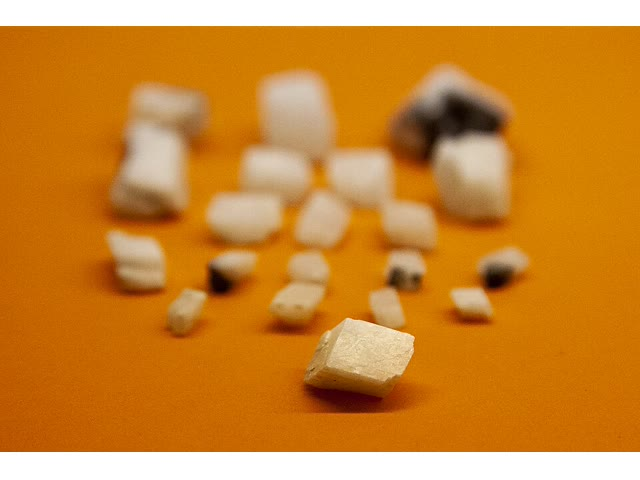
\includegraphics[width=\linewidth]{images/book3/b1-mineral-calcite-rhombs.jpg}

{\scriptsize कैल्साइट विदलन के समचतुर्भुज। फ़ोटो: जियोवाना कानु और एवा सैंटिनी, CC BY 4.0 (विकिमीडिया कॉमन्स)।}
\end{minipage}
\end{inthelab}

\begin{omfigure}
\setlength{\tabcolsep}{2pt}
\begin{tabular}{ccc}
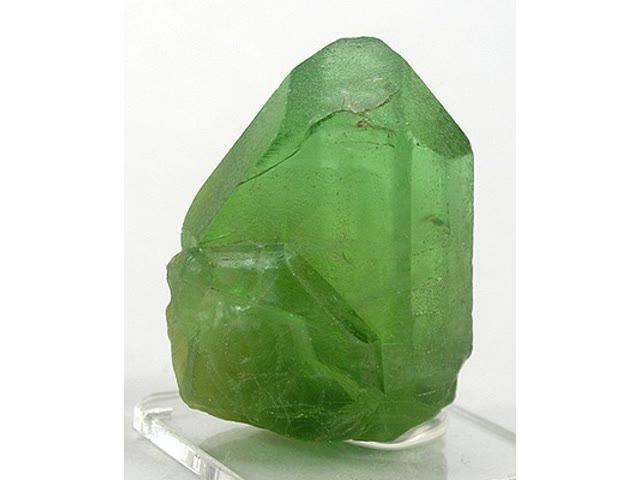
\includegraphics[width=0.31\linewidth]{images/book3/b1-mineral-olivine.jpg} &
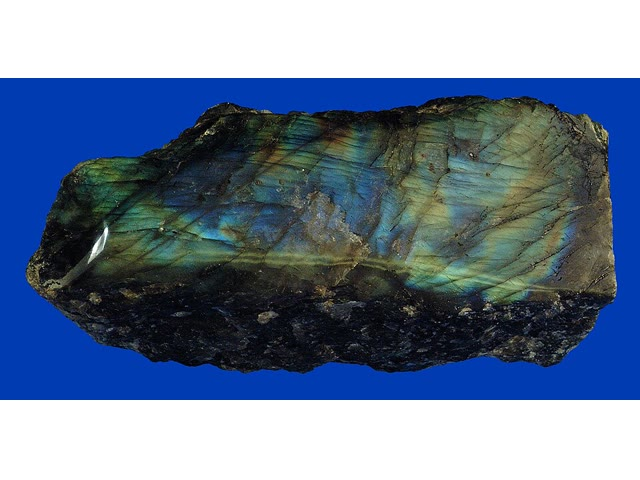
\includegraphics[width=0.31\linewidth]{images/book3/b1-mineral-plagioclase.jpg} &
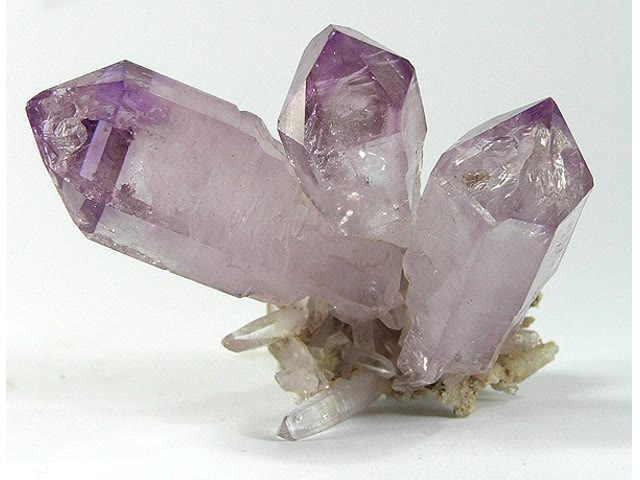
\includegraphics[width=0.31\linewidth]{images/book3/b1-mineral-quartz.jpg} \\
{\small (क) \omterm{def:b1:rock-forming-minerals:groups}{ओलिवीन}} & {\small (ख) \omterm{def:b1:rock-forming-minerals:groups}{प्लैजियोक्लेज़} (लैब्रेडोराइट)} & {\small (ग) स्फटिक (एमेथिस्ट)} \\[4pt]
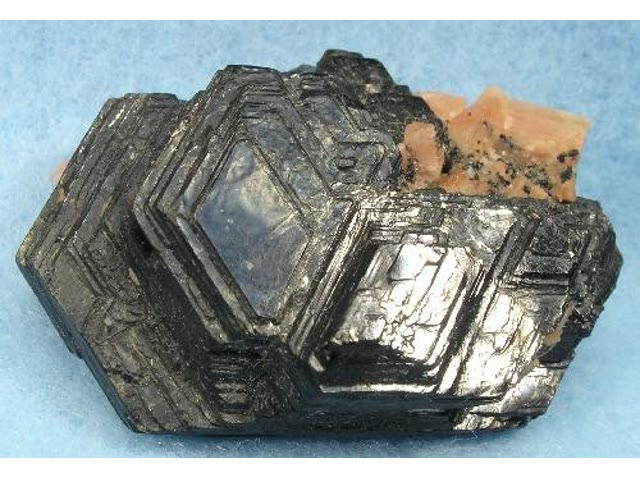
\includegraphics[width=0.31\linewidth]{images/book3/b1-mineral-biotite.jpg} &
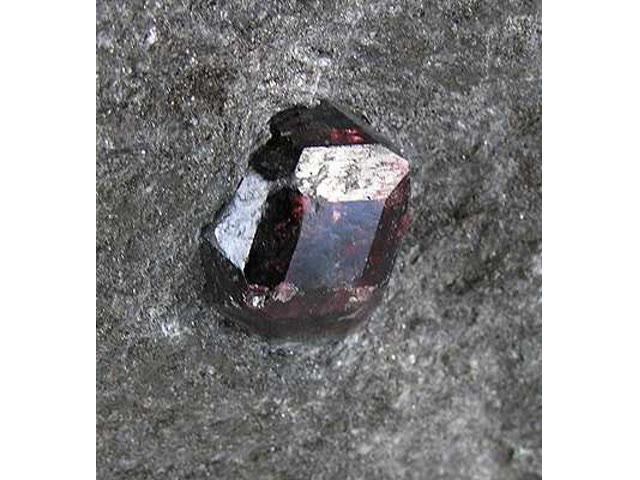
\includegraphics[width=0.31\linewidth]{images/book3/b1-mineral-garnet.jpg} &
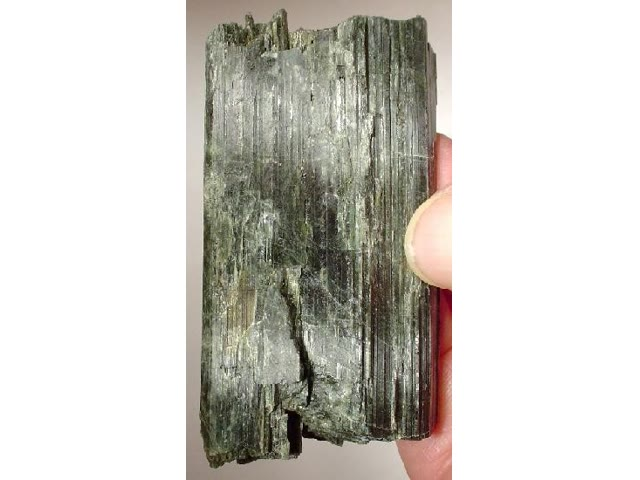
\includegraphics[width=0.31\linewidth]{images/book3/b1-mineral-hornblende.jpg} \\
{\small (घ) ऑर्थोक्लेज़ पर बायोटाइट} & {\small (ङ) \omterm{def:b1:rock-forming-minerals:groups}{गार्नेट} (अल्माँडीन)} & {\small (च) हॉर्नब्लेंड} \\
\end{tabular}
\medskip
\medskip
% ledger: commons:min-olivine, commons:min-plagioclase, commons:min-quartz, commons:min-biotite, commons:min-garnet, commons:min-hornblende

{\small छह शैल-निर्माता \omterm{def:b1:rock-forming-minerals:mineral}{खनिज}: (क) एक रत्न-ओलिवीन क्रिस्टल; (ख) \omterm{def:b1:rock-forming-minerals:groups}{प्लैजियोक्लेज़} की एक पॉलिश की गई पट्टी, जिसमें लैब्रेडोराइट
के रंगों का खेल दिखता है; (ग) स्फटिक के क्रिस्टल, शीर्षों पर पिरामिड वाले छह-पार्श्वीय स्तंभ; (घ) ऑर्थोक्लेज़ के एक
क्रिस्टल पर बायोटाइट के पत्रकों की एक पुस्तक; (ङ) अपने मैट्रिक्स में एक अल्माँडीन \omterm{def:b1:rock-forming-minerals:groups}{गार्नेट} क्रिस्टल; (च) एक हॉर्नब्लेंड
स्तंभ। फ़ोटो (क), (ग)--(च) रॉबर्ट एम॰ लेविंस्की, CC BY-SA 3.0; (ख) ट्विला बेकर, CC0 (विकिमीडिया कॉमन्स)।}
\end{omfigure}

\section{अभ्यास}

\begin{exercise}[$\star$]\label{exo:b1:rock-forming-minerals:1}
हर आयन का सिलिकेट वर्ग नाम दीजिए, और हर चतुष्फलक द्वारा साझा कोनों की संख्या $s$ दीजिए: \ce{SiO4^{4-}}, \ce{Si2O7^{6-}},
\ce{Si6O18^{12-}}, \ce{Si2O5^{2-}}, \ce{SiO2}। \ce{SiO3^{2-}} किस वर्ग का हो सकता है?
\end{exercise}

\begin{exercise}[$\star$]\label{exo:b1:rock-forming-minerals:2}
परमाणु भार O \num{15.999}, Si \num{28.085}, Mg \num{24.305} और Fe \qty{55.845}{g.mol^{-1}} के साथ फ़ॉर्स्टेराइट और
फ़ायलाइट के मोलर द्रव्यमान परिकलित कीजिए, फिर घनत्वों \num{3.275} और \qty{4.392}{g.cm^{-3}} से उनके मोलर आयतन।
% ledger: ciaaw:O, ciaaw:Si, ciaaw:Mg, ciaaw:Fe, hom:forsterite, hom:fayalite

\end{exercise}

\begin{exercise}[$\star$]\label{exo:b1:rock-forming-minerals:3}
षट्भुजीय समन्वय में त्रिज्याएँ \ce{Mg^{2+}} \qty{0.72}{\angstrom}, \ce{Fe^{2+}} \qty{0.78}{\angstrom}, \ce{Ni^{2+}}
\qty{0.69}{\angstrom}, \ce{Mn^{2+}} \qty{0.83}{\angstrom} और \ce{Ca^{2+}} \qty{1.00}{\angstrom} हैं। हर एक का
\ce{Mg^{2+}} की त्रिज्या से प्रतिशत अंतर परिकलित कीजिए, और गोल्डश्मिट के नियमों से बताइए कि \omterm{def:b1:rock-forming-minerals:groups}{ओलिवीन} में मैग्नीशियम को
कौन मुक्त रूप से बदल सकता है।
% ledger: shannon:radii, goldschmidt:size

\end{exercise}

\begin{exercise}[$\star$]\label{exo:b1:rock-forming-minerals:4}
ग्रेफ़ाइट और हीरे के घनत्व \num{2.16} और \qty{3.51}{g.cm^{-3}} हैं; कैल्साइट और ऐरागोनाइट \num{2.71} और
\qty{2.93}{g.cm^{-3}}। हर परिवर्तन में घनत्व कितने प्रतिशत बढ़ता है? हर युग्म का कौन-सा \omterm{def:b1:rock-forming-minerals:polymorph}{बहुरूप} अधिक दाब पर बनता है?
% ledger: webmineral:polymorphs, hom:calcite

\end{exercise}

\begin{exercise}[$\star\star$]\label{exo:b1:rock-forming-minerals:5}
\omterm{def:b1:rock-forming-minerals:groups}{प्लैजियोक्लेज़} $\text{An}_{30}$ का \omterm{def:b1:rock-forming-minerals:formula}{संरचनात्मक सूत्र} लिखिए (बड़े स्थलों का \qty{30}{\percent} कैल्शियम से भरा), और जाँचिए
कि वह उदासीन है।
\end{exercise}

\begin{exercise}[$\star\star$]\label{exo:b1:rock-forming-minerals:6}
एक द्वि-शृंखला में आधे चतुष्फलक दो कोने साझा करते हैं और आधे तीन। चार चतुष्फलकों के एक दोहराते समूह के ऑक्सीजन
जोड़-आकृति के पैनल (च) पर सीधे गिनिए, और \cref{prop:b1:rock-forming-minerals:si-o} द्वारा दिए गए सूत्र
\ce{Si4O11^{6-}} की जाँच कीजिए।
\end{exercise}

\begin{exercise}[$\star\star$]\label{exo:b1:rock-forming-minerals:7}
चार ऑक्सीजन पर \omterm{def:b1:rock-forming-minerals:groups}{ओलिवीन} विश्लेषण की पुनर्गणना कीजिए: \qty{40.20}{\percent} \ce{SiO2}, \qty{47.10}{\percent} \ce{MgO},
\qty{12.20}{\percent} \ce{FeO}, \qty{0.40}{\percent} \ce{NiO} (\ce{NiO} का मोलर द्रव्यमान
\qty{74.692}{g.mol^{-1}})। इसका \omterm{def:b1:rock-forming-minerals:formula}{संरचनात्मक सूत्र} दीजिए, उसकी जाँच कीजिए, और उसकी फ़ॉर्स्टेराइट मात्रा दीजिए। फिर दिखाइए
कि फ़ॉर्स्टेराइट मात्रा केवल \ce{MgO} और \ce{FeO} प्रतिशतों से पाई जा सकती है।
\end{exercise}

\begin{exercise}[$\star\star$]\label{exo:b1:rock-forming-minerals:8}
जाँचिए कि मस्कोवाइट \ce{KAl2(Si3Al)O10(OH)2} उदासीन है। उसकी चतुष्फलकों की परतों में तीन सिलिकन के लिए एक
एल्युमिनियम है: इससे प्रति सूत्र-एकक परत को क्या आवेश मिलता है, और कौन-सा आयन उसे संतुलित करता है?
\end{exercise}

\begin{exercise}[$\star\star$]\label{exo:b1:rock-forming-minerals:9}
मोलर आयतन \num{42.96} और \qty{46.40}{cm^3.mol^{-1}} तथा मोलर द्रव्यमान \num{140.691} और \qty{203.771}{g.mol^{-1}} का
उपयोग करके: (क) आदर्श मिश्रण से $\text{Fo}_{50}$ का घनत्व परिकलित कीजिए, और उसकी तुलना \omterm{def:b1:rock-forming-minerals:solid-solution}{अंत्य-सदस्य} घनत्वों के माध्य से
कीजिए; (ख) \qty{3.600}{g.cm^{-3}} घनत्व वाले एक \omterm{def:b1:rock-forming-minerals:groups}{ओलिवीन} की फ़ॉर्स्टेराइट मात्रा ज्ञात कीजिए।
\end{exercise}

\begin{exercise}[$\star\star\star$]\label{exo:b1:rock-forming-minerals:10}
\cref{prop:b1:rock-forming-minerals:ideal-mixing} के संकेतन के साथ दिखाइए कि
\[
  \rho(x) - \bigl(x\rho_1 + (1 - x)\rho_2\bigr) =
  \frac{x(1 - x)(\rho_1 - \rho_2)(V_1 - V_2)}{V(x)} .
\]
इससे निकालिए कि \omterm{def:b1:rock-forming-minerals:groups}{ओलिवीन} का घनत्व अंत्य-सदस्यों के बीच की सीधी रेखा से ऊपर है, और $\text{Fo}_{50}$ पर अंतर परिकलित कीजिए।
\end{exercise}

\begin{exercise}[$\star\star\star$]\label{exo:b1:rock-forming-minerals:11}
एक गैब्रो के एक \omterm{def:b1:rock-forming-minerals:groups}{प्लैजियोक्लेज़} से \qty{54.10}{\percent} \ce{SiO2}, \qty{28.90}{\percent} \ce{Al2O3}, \qty{11.20}{\percent} \ce{CaO},
\qty{5.10}{\percent} \ce{Na2O} और \qty{0.30}{\percent} \ce{K2O} मिलते हैं (मोलर द्रव्यमान \num{60.083}, \num{101.961}, \num{56.077},
\num{61.979}, \qty{94.195}{g.mol^{-1}})। इसकी आठ ऑक्सीजन पर पुनर्गणना कीजिए; जाँचिए कि चतुष्फलकीय स्थल (Si + Al) 4 परमाणु
और बड़ा स्थल (Ca + Na + K) 1 रखते हैं; $\mathrm{Al} - 1$ की Ca से तुलना करके \omterm{def:b1:rock-forming-minerals:substitution}{युग्मित प्रतिस्थापन} जाँचिए; और एनॉर्थाइट
मात्रा $100\,\mathrm{Ca}/(\mathrm{Ca} +
\mathrm{Na} + \mathrm{K})$ दीजिए।
\end{exercise}

\begin{exercise}[$\star\star\star$]\label{exo:b1:rock-forming-minerals:12}
एक माइक्रोप्रोब \ce{Fe^{2+}} और \ce{Fe^{3+}} में अंतर नहीं कर सकता और सारा लोहा \ce{FeO} के रूप में देता है। (क) दिखाइए
कि इस प्रकार विश्लेषित शुद्ध मैग्नेटाइट \ce{Fe3O4} का योग \qty{93.09}{\percent} है। (ख) इस विश्लेषण की चार ऑक्सीजन पर
पुनर्गणना कीजिए, और बताइए कि चार ऑक्सीजन पर तीन धनायन वाले \omterm{def:b1:rock-forming-minerals:mineral}{खनिज} के लिए परिणाम क्यों असंभव है। (ग) इसके बजाय तीन
धनायनों पर पुनर्गणना कीजिए, और सूत्र के उदासीन होने की अपेक्षा से \ce{Fe^{2+}} और \ce{Fe^{3+}} की संख्याएँ ज्ञात कीजिए।
(घ) विश्लेषण को \ce{FeO} और \ce{Fe2O3} के रूप में पुनः व्यक्त कीजिए, और नया योग दीजिए।
\end{exercise}

\section{समस्या: बेसाल्ट का एक ओलिवीन}

\begin{problem}[{सप्ताहांत समस्या --- ओलिवीन के एक माइक्रोप्रोब विश्लेषण की पुनर्गणना, उसके सूत्र का लिखना और जाँचना, और
उसका संघटन, घनत्व और एक घन मीटर बेसाल्ट में उसका द्रव्यमान ज्ञात करना}]
\label{pb:b1:rock-forming-minerals:1}
% invented analysis: figdata/bachelor-1/solid_solution.py (OLIVINE_WT); values: calc/ch07.py
% ledger: ciaaw:O, ciaaw:Si, ciaaw:Mg, ciaaw:Fe, ciaaw:Mn, ciaaw:Ni, ciaaw:Ca, hom:forsterite, hom:fayalite, shannon:radii
बेसाल्ट के हरे क्रिस्टल \omterm{def:b1:rock-forming-minerals:groups}{ओलिवीन} हैं। उनमें से एक का माइक्रोप्रोब विश्लेषण ऑक्साइडों के भार प्रतिशत में देता है:
\begin{center}
\small
\begin{tabular}{lcccccc}
\hline
ऑक्साइड & \ce{SiO2} & \ce{FeO} & \ce{MnO} & \ce{MgO} & \ce{NiO} & \ce{CaO} \\
भार \% & 39.50 & 16.53 & 0.23 & 43.32 & 0.20 & 0.22 \\
\hline
\end{tabular}
\end{center}
परमाणु भार O \num{15.999}, Si \num{28.085}, Fe \num{55.845}, Mn
\num{54.938}, Mg \num{24.305}, Ni \num{58.693}, Ca \qty{40.078}{g.mol^{-1}} हैं।
फ़ॉर्स्टेराइट का घनत्व \qty{3.275}{g.cm^{-3}} और फ़ायलाइट का
\qty{4.392}{g.cm^{-3}} है।
\medskip
\noindent\textbf{भाग I --- ऑक्साइडों से धनायनों तक।}
\begin{enumerate}
  \item छह ऑक्साइडों के मोलर द्रव्यमान परिकलित कीजिए।
  \item विश्लेषण का योग परिकलित कीजिए। \qty{97}{\percent} का योग क्या सुझाता?
  \item \qty{100}{g} \omterm{def:b1:rock-forming-minerals:groups}{ओलिवीन} में हर ऑक्साइड के मोल परिकलित कीजिए।
  \item उनमें निहित ऑक्सीजन के मोल, और उनका योग परिकलित कीजिए।
  \item हर धनायन के मोल परिकलित कीजिए।
  \item वह गुणक परिकलित कीजिए जो ऑक्सीजन को चार तक लाता है।
  \item प्रति चार ऑक्सीजन हर तत्व के परमाणुओं की संख्या दीजिए, तीन दशमलव तक।
\end{enumerate}

\medskip
\noindent\textbf{भाग II --- संरचनात्मक सूत्र।}
\begin{enumerate}[resume]
  \item \omterm{def:b1:rock-forming-minerals:groups}{ओलिवीन} में प्रति चार ऑक्सीजन एक चतुष्फलकीय और दो अष्टफलकीय स्थल हैं। सिलिकन के अलावा अन्य धनायनों का योग परिकलित
        कीजिए, और दोनों स्थल-योगों की आदर्श सूत्र से तुलना कीजिए।
  \item \omterm{def:b1:rock-forming-minerals:groups}{ओलिवीन} का \omterm{def:b1:rock-forming-minerals:formula}{संरचनात्मक सूत्र} लिखिए।
  \item जाँचिए कि सूत्र उदासीन है, और समझाइए कि यह जाँच, प्रश्न 8 की जाँच के विपरीत, विफल क्यों नहीं हो सकती थी।
  \item आयनिक त्रिज्याओं (\ce{Mg^{2+}} \qty{0.72}{\angstrom}, \ce{Fe^{2+}} \qty{0.78}{\angstrom}, \ce{Ni^{2+}}
        \qty{0.69}{\angstrom}, \ce{Mn^{2+}} \qty{0.83}{\angstrom}, \ce{Ca^{2+}} \qty{1.00}{\angstrom}, सभी षट्भुजीय) का उपयोग करके
        समझाइए कि \omterm{def:b1:rock-forming-minerals:groups}{ओलिवीन} में निकेल आम क्यों है और कैल्शियम दुर्लभ क्यों।
  \item माइक्रोप्रोब सारा लोहा \ce{FeO} के रूप में देता है। समझाइए कि प्रश्न 7 में मिले धनायनों का कुल योग यह क्यों दिखाता है
        कि \omterm{def:b1:rock-forming-minerals:groups}{ओलिवीन} में कोई महत्वपूर्ण \ce{Fe^{3+}} नहीं है।
\end{enumerate}

\medskip
\noindent\textbf{भाग III --- संघटन।}
\begin{enumerate}[resume]
  \item फ़ॉर्स्टेराइट मात्रा $\mathrm{Fo} = 100\,\mathrm{Mg}/(\mathrm{Mg} +
        \mathrm{Fe})$ एक दशमलव तक परिकलित कीजिए।
  \item \omterm{def:b1:rock-forming-minerals:groups}{ओलिवीन} की \omterm{def:b1:rock-forming-minerals:formula}{Mg संख्या} क्या है? वह यहाँ फ़ॉर्स्टेराइट मात्रा के बराबर क्यों है?
  \item \omterm{def:b1:rock-forming-minerals:groups}{ओलिवीन} को एक द्विआधारी \omterm{def:b1:rock-forming-minerals:solid-solution}{ठोस विलयन} $\mathrm{Fo}_x\mathrm{Fa}_{1-x}$ के रूप में लिखिए, Mn, Ni और Ca की उपेक्षा करते
        हुए, और उसके अष्टफलकीय स्थलों में लोहे वाले स्थलों का अनुपात दीजिए।
  \item दिखाइए कि फ़ॉर्स्टेराइट मात्रा केवल \ce{MgO} और \ce{FeO} प्रतिशतों से परिकलित की जा सकती है, प्रश्न 6 के गुणक के
        बिना, और उसे कीजिए।
  \item उसी लावा में बाद में उगा एक \omterm{def:b1:rock-forming-minerals:groups}{ओलिवीन} \qty{40.5}{\percent} \ce{MgO} और \qty{20.0}{\percent} \ce{FeO} रखता है। उसकी
        फ़ॉर्स्टेराइट मात्रा परिकलित कीजिए। कौन-सा \omterm{def:b1:rock-forming-minerals:groups}{ओलिवीन} लोहे में अधिक समृद्ध है?
\end{enumerate}

\medskip
\noindent\textbf{भाग IV --- घनत्व और द्रव्यमान।}
\begin{enumerate}[resume]
  \item फ़ॉर्स्टेराइट और फ़ायलाइट के मोलर द्रव्यमान और मोलर आयतन परिकलित कीजिए (मोलर आयतन दो दशमलव तक)।
  \item \omterm{def:b1:rock-forming-minerals:groups}{ओलिवीन} को प्रश्न 15 के द्विआधारी $\mathrm{Fo}_x\mathrm{Fa}_{1-x}$ के रूप में लेते हुए, $x$ को तीन दशमलव तक पूर्णांकित
        करके, उसका मोलर द्रव्यमान और आदर्श मिश्रण से मोलर आयतन परिकलित कीजिए।
  \item उससे उसका घनत्व, तीन दशमलव तक, निकालिए।
  \item उसकी तुलना \omterm{def:b1:rock-forming-minerals:solid-solution}{अंत्य-सदस्य} घनत्वों के बीच की सीधी-रेखा अंतर्वेशन से कीजिए।
  \item बेसाल्ट में आयतन से \qty{12}{\percent} \omterm{def:b1:rock-forming-minerals:groups}{ओलिवीन} है। एक घन मीटर बेसाल्ट में \omterm{def:b1:rock-forming-minerals:groups}{ओलिवीन} का कितना द्रव्यमान है?
  \item बेसाल्ट का घनत्व \qty{2.95}{g.cm^{-3}} है। द्रव्यमान से \omterm{def:b1:rock-forming-minerals:groups}{ओलिवीन} का अनुपात क्या है?
  \item \omterm{def:b1:rock-forming-minerals:groups}{ओलिवीन} की फ़ॉर्स्टेराइट मात्रा क्या है, पूरे प्रतिशत तक पूर्णांकित?
\end{enumerate}
\end{problem}
